%%%%%%%%%%%%%%%%%%%%%%%%%%%%%%%%%%%%%%%%%
% Short Sectioned Assignment
% LaTeX Template
% Version 1.0 (5/5/12)
%
% This template has been downloaded from:
% http://www.LaTeXTemplates.com
%
% Original author:
% Frits Wenneker (http://www.howtotex.com)
%
% License:
% CC BY-NC-SA 3.0 (http://creativecommons.org/licenses/by-nc-sa/3.0/)
%
%%%%%%%%%%%%%%%%%%%%%%%%%%%%%%%%%%%%%%%%%

%----------------------------------------------------------------------------------------
%	PACKAGES AND OTHER DOCUMENT CONFIGURATIONS
%----------------------------------------------------------------------------------------

\documentclass[paper=a4, fontsize=11pt]{scrartcl} % A4 paper and 11pt font size

\usepackage[T1]{fontenc} % Use 8-bit encoding that has 256 glyphs
\usepackage{fourier} % Use the Adobe Utopia font for the document - comment this line to return to the LaTeX default
\usepackage[english]{babel} % English language/hyphenation
\usepackage{amsmath,amsfonts,amsthm} % Math packages

\usepackage{lipsum} % Used for inserting dummy 'Lorem ipsum' text into the template

\usepackage{sectsty} % Allows customizing section commands
\allsectionsfont{\centering \normalfont\scshape} % Make all sections centered, the default font and small caps

\usepackage{graphicx} %Figures

\usepackage{fancyhdr} % Custom headers and footers
\pagestyle{fancyplain} % Makes all pages in the document conform to the custom headers and footers
\fancyhead{} % No page header - if you want one, create it in the same way as the footers below
\fancyfoot[L]{} % Empty left footer
\fancyfoot[C]{} % Empty center footer
\fancyfoot[R]{\thepage} % Page numbering for right footer
\renewcommand{\headrulewidth}{0pt} % Remove header underlines
\renewcommand{\footrulewidth}{0pt} % Remove footer underlines
\setlength{\headheight}{13.6pt} % Customize the height of the header

\numberwithin{equation}{section} % Number equations within sections (i.e. 1.1, 1.2, 2.1, 2.2 instead of 1, 2, 3, 4)
\numberwithin{figure}{section} % Number figures within sections (i.e. 1.1, 1.2, 2.1, 2.2 instead of 1, 2, 3, 4)
\numberwithin{table}{section} % Number tables within sections (i.e. 1.1, 1.2, 2.1, 2.2 instead of 1, 2, 3, 4)

\setlength\parindent{0pt} % Removes all indentation from paragraphs - comment this line for an assignment with lots of text

%----------------------------------------------------------------------------------------
%	TITLE SECTION
%----------------------------------------------------------------------------------------

\newcommand{\horrule}[1]{\rule{\linewidth}{#1}} % Create horizontal rule command with 1 argument of height

\title{	
\normalfont \normalsize 
\textsc{Aalborg University} \\ [25pt] % Your university, school and/or department name(s)
\horrule{0.5pt} \\[0.4cm] % Thin top horizontal rule
\huge Worksheet - Rules \\ % The assignment title
\horrule{2pt} \\[0.5cm] % Thick bottom horizontal rule
}

\date{\normalsize\today} % Today's date or a custom date

\begin{document}

\maketitle % Print the title

%----------------------------------------------------------------------------------------
%	PROBLEM 1
%----------------------------------------------------------------------------------------

\section{Designing rules for VR environment}

%why have we done this

\begin{align} 
\begin{split}
E = M * C^2
\end{split}					
\end{align}

To ensure realism and to estimate functionality of the virtual reality simulation a set of rules for the system should be drawn. The core rules can be separated into three primary groups; the system, the users, and the virtual equipment. The mindmap of these rules can be seen below:

\begin{figure}
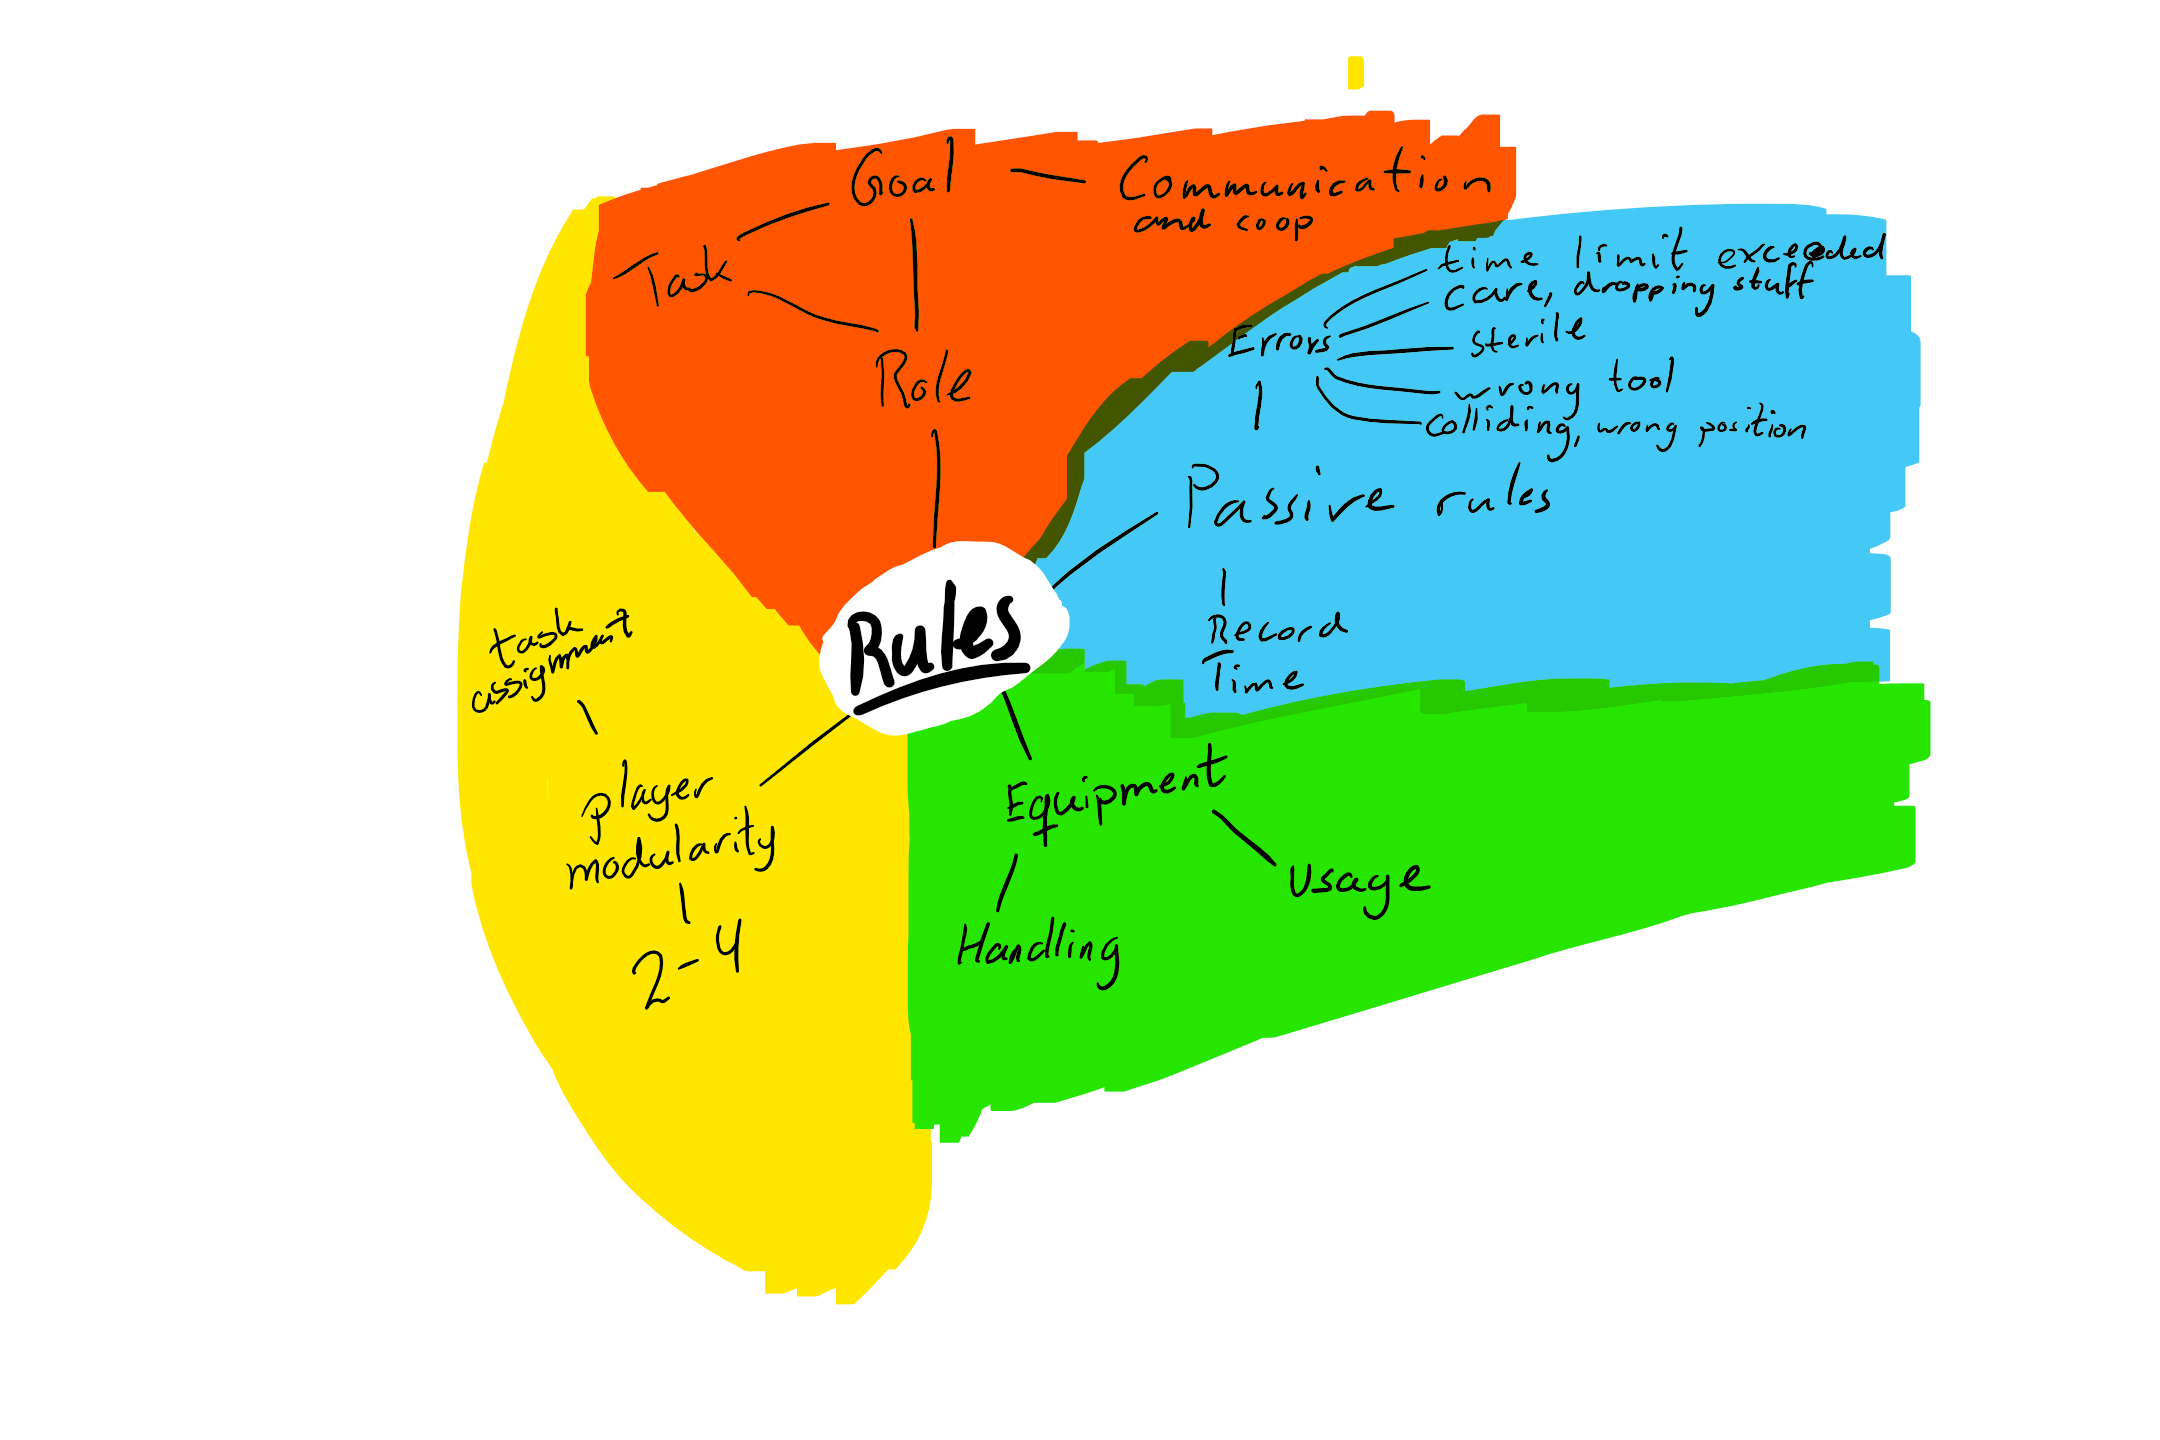
\includegraphics[scale=1]{brainstorm rules.png}
\caption{Mindmap}
\label{fig:Rules}
\end{figure}

\subsection{The System}
The rules set for the system consists of both the player modality and the passive rules. It is important that the system is not limited to four players but should also be able to adapt to as low as two players. As such, the tasks for the users should be adapted to the amount of colleagues present.

The passive rules functions as a way to quantify the effectiveness of the sessions. It should therefore measure the time it takes to complete the individual tasks as well as alert the system and the users if any errors are made. The procedures that will be subject to errors would be some of the essential tasks that the users have to perform based upon the task-list given by Jane Petersson. For example, interactive with non-sterile equipment while being sterile.

\subsection{The User}
The users in the scene should be designated a specific role which entails different tasks depending on the amount of users in the current session. While completing the individual tasks is important, the primary focus of this exercise is to complete the overall task of saving the patient as one unit. This means that communication and cooperation is very important to the success of this goal.

\subsection{The Equipment}
The rules for the equipment is based on the observations and interview with Jane. These rules entails how the equipment should be used and handled by the users. As most of the equipment is only used for one specific use, it important that the users are aware of that specific use.

%----------------------------------------------------------------------------------------

\end{document}